\section{Machine Learning based Method}
Machine Learning is a popular approach in Sentiment Analysis. Pang et al. were one of the first to employ and compare the use of different machine learning classifiers, without using any prior knowledge. Their classifiers worked in the movie review domain, where they were able to achieve high accuracy \cite{pang-etal-2002-thumbs}. Go et al. proved that machine learning classifiers also achieved high accuracy in the Twitter domain.


\begin{figure}
    \centering
    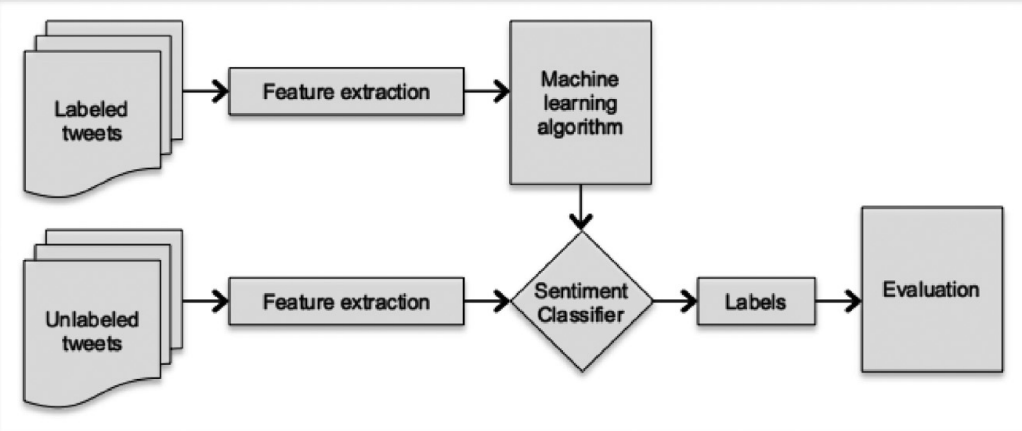
\includegraphics[scale=0.5]{Images/ML_approach.png}
    \caption{Caption}
    \label{fig:ml_approach}
\end{figure}

\begin{figure}
    \centering
    \tikzset{
  every shadow/.style={
    fill=none,
    shadow xshift=0pt,
    shadow yshift=0pt}
}
\tikzset{module/.append style={top color=\col,bottom color=\col}}

\smartdiagramset{uniform color list=white for 6 items,
    back arrow disabled=true, module minimum width=2cm,
    module minimum height=2cm,
    module x sep=3cm,
    text width=2cm,
    uniform arrow color=true,
    arrow color=black,
    additions={
        additional item shape=rectangle,
        additional item offset=0.5cm,
        additional item width=4cm,
        additional item height=2cm,
        additional item text width=4cm,
        additional item fill color=white!20,
        additional item border color=black,
        additional arrow color=gray,
        additional arrow tip=stealth,
        additional arrow line width=1pt
      }
    }
    \smartdiagramadd[flow diagram:horizontal]{Tokenization, Stop Word Filtering, URL/Hashtag Removal, Stemming, Feature Selection, Classification}
    {below of module5/Unigrams vs. Bigrams \\ Word Frequency vs. Presence} 
    \smartdiagramconnect{->}{module5/additional-module1}
    \vspace{25mm}

   \caption{Caption}
    \label{fig:my_label}
\end{figure}

\TODO{better: sources, more reasoning, stats, citation, etc. --> WHY did you choose this approach?, figure see Lin thesis}

\subsection{Tokenization}
\TODO{more?}

Tokenization refers to the extraction of words out of a tweet/sentence \cite{DBLP:journals/csur/GiachanouC16}. In this thesis, tweets are tokenized based on whitespace. \TODO{ngram here!}
\subsection{Stop Word Filtering}
Because every word is treated as an attribute, some words can be removed in advance to improve both data sparsity and the feature size. Words with low impact on the sentiment of a sentence, such as "the" and "is", are referred to as Stop words and can thus be ignored \cite{DBLP:journals/csur/GiachanouC16}. Although there are pre-compiled lists of Stop Words, these often are outdated and not Twitter specific. Additionally, Saif et al. observed that the usage of pre-compiled lists reduced the accuracy of classification performance and recommended a dynamic solution, which considers the number of times a word appears over the data set \cite{data_sparsity}. 

\subsection{URL/Hashtag Removal}
Tweets often contain URLs of the media, article, etc. the tweet is concerned with. Because these links in itself don't affect the sentiment, they are too ignored. Additionally, tweets often contain a hashtag, which indicates that the tweet is concerned with specific topic. The hashtag character "\#" is removed, to not differentiate between words such as \#good and good and thus further reduce data sparsity and feature size.
\subsection{Stemming}
Tweets as an informal message often contain misspelled or otherwise modified words \cite{DBLP:journals/csur/GiachanouC16}. By using word stemming, which, according to Lovins, "reduces all words with the same root (or, if prefixes are left
untouched, the same stem) to a common form" \cite[p.~22]{Lovins1968DevelopmentOA}, different cases or spellings of the same word can be reduced to one common feature, which, again, reduces data sparsity.

\subsection{Feature Selection}
The machine-learning classifier relies on features, also called attributes, which have to be extracted from the training data. In Twitter, these features most often are syntactic features, such as words. Here, the approaches also differentiate between a feature consisting of only one word, also called unigram, or two (bigram) or more words (n-gram). Additionally, the assigned value also differs between using the binary presence of a word, or its frequency in a tweet \cite{DBLP:journals/csur/GiachanouC16}. In this thesis, all approaches are considered.

\subsection{Classification}
Once the training data has been preprocessed and turned into features, the task of training the models can begin. The classifiers chosen are Naive Bayes using the Gaussian Distribution, Naive Bayes using the multinomial Distribution, Random Forest, Logistic Regression and Support Vector Machine. Because the classifiers may have different runtimes, each classifier is first evaluated using a small subset of training data, to obtain a first impression of the training runtime. After this, the data size is gradually increased, until the entire data set was used, or the process becomes too resource intensive. Once the appropiate training size is found, the parameters of each classifier are evaluated, to improve both performance and accuracy. If the performance can be improved, the training size is adjusted accordingly. Once the optimal parameters and training size are found, the classifiers are evaluated and compared. To facilitate a better comparison, the classifiers are evaluated both using their maximum training size, as well as the same minimum training size.

The following sections explain each machine-learning method in more detail.

    \subsubsection{Naive Bayes}
        Naive Bayes is a probabilistic classification model. It is based on the Bayes theorem, which is shown in Equation \eqref{eq:bayes}:
        \begin{equation}
            \label{eq:bayes}
            P(c_j|d_i) = \frac{P(c_j) * P(d_i|c_j)}{P(d_i)}
        \end{equation}
        where $c$ is the class label and $d$ is a set of attribute values \cite{DBLP:books/aw/TanSKK2019}. 
        
        \TODO{Zitat abändern}

        Bayes theorem allows to calculate the posterior probability $P(c|d)$, which Tan et al. describe as "the probability of observing a class label $c$ for a data instance given its set of attribute values $d$" \cite[p.~418]{DBLP:books/aw/TanSKK2019}. 

        To calculate the posterior probability, the class conditional probability $P(d|c)$ is needed, which describes the probability of observing a set of attribute values given a class. One approach to calculate the class conditional probability outlined by Tan et al. is to ''consider the fraction of training instances of a given class for every possible combination of attribute values'' \cite[p.~419]{DBLP:books/aw/TanSKK2019}. With a large number of attributes and values, this method becomes computationally infeasible due to the exponential growth of combinations \cite{DBLP:books/aw/TanSKK2019}.

        Due to this, the Naive Bayes assumption is employed to estimate the class conditional probability. Naive Bayes uses conditional independence, which states that attribute values are only dependent on the class label and not each other. Thus, the class conditional probability can be calculated by using Equation \eqref{eq:naive_assumption}:
        \begin{equation}
            \label{eq:naive_assumption}
            P(d_i|c_j) = \prod_{t=1}^{n}P(w_{t}|c_j)
        \end{equation}
        with $d_i$ containing $n$ attributes $\{w_1,w_2,...,w_t\}$ \cite{DBLP:books/aw/TanSKK2019}.

        Furthermore, $P(d)$ remains constant for every class label $c$, so the class that maximizes Equation \eqref{eq:naive_final} is chosen: 
        \begin{equation}
            \label{eq:naive_final}
            P(c_j|d_i)\propto P(c_j)\prod_{t=1}^{n}P(w_{t}|c_j) 
        \end{equation}   
        
        \TODO{P(c) eingehen}
        
        There are different models on how to implement the Naive Bayes assumption for text classification. In this thesis, the Gaussian Naive Bayes and Multinomial Naive Bayes are discussed. 
        
        The Gaussian Naive Bayes assumes that numeric attributes, such as word count, are distributed according to the normal distribution, also called Gaussian distribution \cite{nb_gauss}. According to Evans et al., "it was originally developed as an approximation to the binomial distribution when the number of trials is large and the Bernoulli probability p is not close to 0 or 1". \cite[p.~143]{evans2011statistical}. It is described by two parameters, the mean $\mu$ and the standard deviation $\sigma$ \cite{evans2011statistical}. Applied to Naive Bayes, it results in Equation \eqref{nb:gauss}:
        \begin{equation}
        \label{nb:gauss}
            P(w_t = v|c_j) = \frac{1}{\sqrt{2\pi}\sigma}e^{-\frac{(v.\mu)^2}{2\sigma^2}},
        \end{equation}
        with $v$ denoting the number of times $w_t$ appears in the to be classified document.
        
        In order to calculate Equation \eqref{nb:gauss}, the mean $\mu$ and the standard deviation $\sigma$ have to be estimated for each numeric attribute given the class. Using maximum likelihood estimation, we estimate these two parameters using the training data. Once these two parameters are estimated for every attribute and class, unknown instances can be classified using Equation \eqref{nb:gauss} in conjunction with Equation \eqref{eq:naive_final}.
        
        According to McCallum and Nigan, "the multinomial model captures word frequency information in documents" \cite[p.~3]{Mccallum1998}. In this case, a document is represented by a tweet. By considering not only if a word is present but also how often it is present, the additional information may have an advantage. They describe the document as being "an ordered sequence of word events, drawn from the same vocabulary V" \cite[p.~3]{Mccallum1998}, with its length being independent of class. Using Naive Bayes, we assume that every word event is independent.
        
        \TODO {Gleichung?}
        
        According to Evans et al., "the multinomial variate is a multidimensional generalization of the binomial. Consider a trial that can result in only one of $k$ possible distinct outcomes, labeled $A_i, i = 1,...,k$. The outcome $A_i$ occurs with probability $p_i$. The multinomial distribution relates to a set of n-independent trials of this type." \cite[p.~135]{evans2011statistical}.
        
        Applying this to the model, McCallum and Nigan state that "each document $d_i$ is drawn from a multinomial distribution of words with as many independent trials as the length of $d_i$" \cite[p.~3]{Mccallum1998}. Using the multinomial distribution, the class conditional probability can then be calculated using Equation \eqref{eq:multinomial_bayes}:
        \begin{equation}
            \label{eq:multinomial_bayes}
                P(d_i|c_j) = P(|d_i|)|d_i|!\prod_{t=1}^{|V|}\frac{P(w_t|c_j)^{N_{i_t}}}{N_{i_t}!}
        \end{equation}
        
        with the document $d_i$ containing $|V|$ words $w_t$, $N_{i_t}$ being the number of times $w_t$ appears in $d_i$ and $c_j$ describing a class \cite{Mccallum1998}. 
        
        To estimate $P(w_t|c_j)$, the probability of a word $w_t$ given a class $c_j$, training instances are used to count the number of times a word appears in a class in Equation \eqref{eq:prob_word}:
        \begin{equation}
            \label{eq:prob_word}
                P(w_t|c_j) = \frac{1 + \sum_{i=1}^{|D|}N_{it} P(c_j|d_i)}{|V| + \sum_{s=1}^{|V|} \sum_{i=1}^{|D|}N_{is} P (c_j|d_i)} 
        \end{equation}
        with $D$ containing labeled training documents $d_i$, $N_{it}$ describing the number of times $w_t$ appears in document $d_i$ and $|V|$ containing all words.
        Equation \eqref{eq:prob_word} contains the posterior probability $P(c_j|d_i)$, which is the probability we want to calculate for unknown documents. Because we here have labeled training documents, we know the class label, thus resulting in the posterior probability shown in Equation \eqref{eq:post_prob}:
        \begin{equation}
                \label{eq:post_prob}
                P(c_j|d_i)= 
                \begin{dcases}
                1,& \text{if } d_i \text{ has the class label } c_j \\
                0,              & \text{otherwise}
        \end{dcases}
        \end{equation}
        Because of Equation \eqref{eq:post_prob}, Equation \eqref{eq:prob_word} only sums up the number of occurrences of a word in instances of a single class, thus it can be simplified into Equation \eqref{eq:prob_word_simpler}:
                \begin{equation}
            \label{eq:prob_word_simpler}
                P(w_t|c_j) = \frac{1 + count(w_t, c_j)}{|V| + \sum_{s=1}^{|V|}count(w_s|c_j)} 
        \end{equation}

        with $count(w_t|c_j)$ counting the number of times a word $w_t$ appears in all training instances of a class $c_j$.
        
        By using Equation \eqref{eq:prob_word}, we calculate the word probability $P(w_t|c_j$). We utilize this in Equation \eqref{eq:multinomial_bayes} to calculate the class conditional probability $P(d_i|c_j)$ using the multinomial distribution. Finally, this allows us to estimate the posterior probability $P(c|d)$, as shown in Equation \eqref{eq:naive_final}. By selecting the class with the higher posterior probability, the classifier is able to make a prediction.
        
\subsubsection{Random Forest}
        According to Tan et al., Random Forest is an ensemble method that utilizes multiple base classifiers to take a vote on their predictions. The final prediction is then made by either averaging the vote or taking the majority vote. Random Forest applies a set of decorrelated decision trees by implementing two key characteristics.
        
        The first characteristic is Bagging. Each tree is trained by a data set that was sampled from the original training data. Because the sampling is done with replacement and the samples must have the same size as the original training data, the sample will, on average, only contain 63\% of the original data.
        
        The selection of input attributes is the second characteristic. When a tree is being constructed, an attribute must be selected for splitting at each internal node.
        Random Forest randomly chooses a subset of attributes, from which the attribute with the maximum reduction in an impurity measure is chosen.
        
        Through these characteristics, Random Forest reduces the correlation of trees and thus the variance \cite{DBLP:books/aw/TanSKK2019}. In Figure \ref{fig:tree}, a part of a tree generated by a Random Forest classifier can be seen. Here, the existence of a word is used as the attribute for splitting. If, for example, $hurts \geq 0.5$, the word $hurts$ exist in the document that is being analyzed, while $hurts < 0.5$ signifies that the word $hurts$ does not exist.
        
        \begin{figure}[h!]
        \centering
        \begin{tikzpicture}
        [
        grow                    = right,
    sibling distance        = 4em,
    level distance          = 9em,
    edge from parent/.style = {draw, -latex},
    every node/.style       = {font=\footnotesize},
    sloped
  ]
  \node [root] {}
    child { node [dummy] {}
      child { node [dummy] {}
        child { node [dummy] {}
            child { node [env] {$-1.0$}
                edge from parent node [below, align=center] {$studying < 0.5$} }
            child { node [env] {$+1.0$}
                edge from parent node [above] {$studying \geq 0.5$} }
            edge from parent node [below] {$will < 0.5$} }
        child { node [env] {$-1.0$}
                edge from parent node [above] {$will \geq 0.5$} }
        edge from parent node [below] {$hates < 0.5$} }
      child { node [env] {$-1.0$}
              edge from parent node [above, align=center]
                {$hates \geq 0.5$}}
              edge from parent node [above] {$hurts \geq 0.5$} };
\end{tikzpicture}
    \caption{Part of a tree generated by the Random Forest classifier.}
      \label{fig:tree}
\end{figure}
\TODO{satzzeichen nach Gleichung, siehe Buch}
\TODO{citations}
\subsubsection{Logistic Regression}
Logistic Regression calculates the posterior probability $P(c_j|d_i)$ directly, without relying on the class conditional probability like Naive Bayes, which is why it is a probabilistic discriminative model. In a binary model, the class label can be assigned by calculating the odds, as seen in Equation \eqref{eq:logistic_odds}:
        \begin{equation}
            \label{eq:logistic_odds}
                \frac{P(c=1|d)}{P(c=0|d)}
        \end{equation}
If the odds are greater than 1, then the class label 1 can be assigned to document d, otherwise class 0 is assigned. Logistic Regression represents the odds using a linear predictor $z=w^Tx + b$, which results in equation \eqref{eq:logistic_linear}:
        \begin{equation}
            \label{eq:logistic_linear}
                \frac{P(c=1|d)}{P(c=0|d)} = e^z = e^{w^Td+b}
        \end{equation}
with the parameters $w$ and $b$ and $w^t$ signifying the vector transpose \cite{DBLP:books/aw/TanSKK2019}.

By substituting $P(c=0|d)$ with $1 - P(c=1|x)$ and solving for $P(c=1|d)$, we get Equation \eqref{eq:logistic_sigmoid}:
        {\begin{equation}
            \label{eq:logistic_sigmoid}
                P(c=1|d) = \frac{1}{1+e^{-z}} = \sigma(z)
        \end{equation}}
$\sigma(z)$ is called the sigmoid function, whose graph can be seen in Figure \ref{fig:sigmoid}.
        \begin{figure}[h!]
        \centering

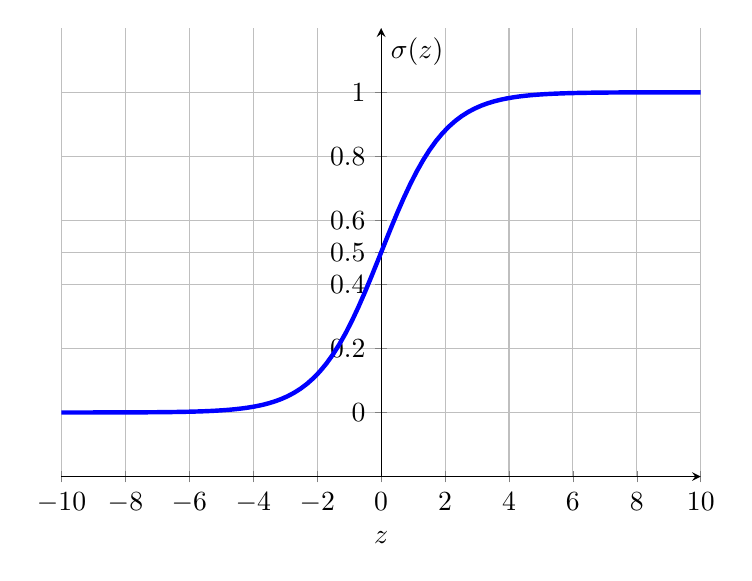
\begin{tikzpicture}
\begin{axis}
[
    grid=major,   
    xmin=-10,
    xmax=10,
    axis x line=bottom,
    ytick={0,.2,.4,.5,.6,.8,1},
    ymax=1.2,
    ymin=-0.2,
    axis y line=middle,
    width=0.8\textwidth,
    height=0.6\textwidth,
    xlabel={$z$},
    ylabel={$\sigma(z)$}
]
    \addplot%
    [
        blue,%
        mark=none,
        samples=100,
        domain=-10:10,
        ultra thick
    ]
    (x,{1/(1+exp(-x))});
\end{axis}
\end{tikzpicture}
    \caption{Plot of sigmoid function $\sigma(z)$.}
      \label{fig:sigmoid}
\end{figure}
As seen in Figure \ref{fig:sigmoid}, $\sigma(z) \geq 0.5$ when $z \geq 0$, so if $z \geq 0$, we assign the instance $d_i$ to the class $c = 1$. Using training instances, the parameters $w$ and $b$ can be learned, and thus the posterior probability $P(c_j|d_i)$ can be estimated \cite{DBLP:books/aw/TanSKK2019}.

\subsubsection{Support Vector Machine}
Tan et al. describe the Support Vector Machine as a discriminative classifier. It is based on a separating hyperplane that, as the name suggests, tries to separate instances of two classes. Furthermore, it uses a subset of the training instances, those that are the hardest to classify, meaning those nearest the boundaries of the classes. These instances are called support vectors \cite{DBLP:books/aw/TanSKK2019}.

The hyperplane can be described by Equation \eqref{eq:hyperplane}:
    \begin{equation}
            \label{eq:hyperplane}
                w^Td + b = 0,
        \end{equation}
    where $d$ represents the attributes and $(w, b)$ are the parameters of the model. 
    
    There can be an indefinite number of hyperplanes, which is why it is necessary to choose one that has good generalization performance, which means that it can handle unseen instances. To do this, the margin of a hyperplane $B_i$ is calculated. To achieve this, two hyperplanes, $B_i1$ and $B_i2$, parallel to $B_i$ are drawn. The distance between the two hyperplanes is the margin of the hyperplane $B_i$ \cite{DBLP:books/aw/TanSKK2019}.
    \begin{figure}
        \centering
        \caption{\TODO{source}
        \label{fig:svm}
        }
        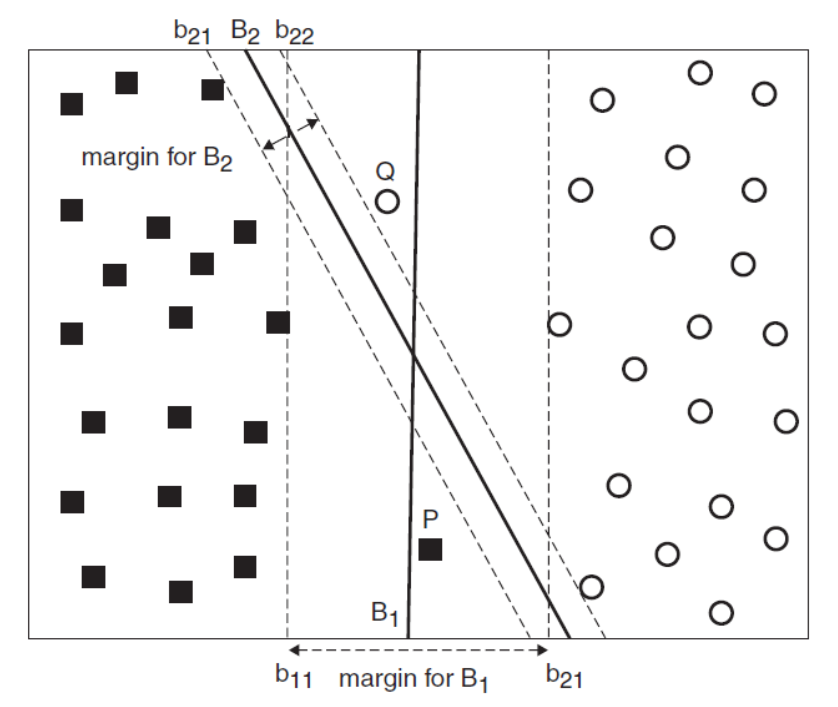
\includegraphics[scale=0.8]{Images/SVM_image.png}
    \end{figure}
    
    By choosing the hyperplane with the maximum margin, the classifier can allow for slight changes in data without immediately crossing onto the other side.
    
    In Figure \ref{fig:svm}, the data can be separated by a linear hyperplane. This is not always the case, which is why nonlinear SVM transform their input data $x$ into a new attribute space $\phi(x)$, in which a linear hyperplane can be constructed. Projected into the original attribute space, this hyperplane is a nonlinear decision boundary \cite{DBLP:books/aw/TanSKK2019}.
    